\documentclass[12pt]{article}
\usepackage[a4paper,margin=1in]{geometry}
\usepackage{amsmath,amssymb,amsthm,mathtools}
\usepackage{graphicx}
\usepackage[hidelinks]{hyperref}
\usepackage{microtype}
\graphicspath{{figures/}}

\newtheorem{theorem}{Theorem}
\newtheorem{lemma}{Lemma}
\newtheorem{corollary}{Corollary}
\theoremstyle{remark}
\newtheorem{remark}{Remark}

\title{\textbf{NB/BD Stability via a Weighted Hilbert Lemma (v3.0, Orthodox Edition)}}
\author{Serabi}
\date{October 2025}

\begin{document}
\maketitle

\begin{abstract}
This orthodox v3.0 note consolidates the Nyman--Beurling/B\'aez\hbox{-}Duarte (NB/BD) stability line.
We rely on a weighted Hilbert-type lemma for M\"obius-weighted coefficients that suppresses off-diagonal
mass by a power of $\log N$. The figures included are the same illustrative plots previously generated
in this series and are reused here for completeness; they do not constitute a proof of the Riemann Hypothesis.
\end{abstract}

\section{Weighted Hilbert Lemma (Sketch)}
Let $a_n=\mu(n)\,v(n/N)\,q(n)$ where $v\in C_0^\infty(0,1)$ and $q$ is slowly varying. With
\begin{equation}
K_{mn}=e^{-\frac12|\log(m/n)|}=\min\!\Big\{\sqrt{m/n},\sqrt{n/m}\Big\},
\end{equation}
one shows by a logarithmic-band decomposition, the weighted discrete Hilbert inequality, smooth-cutoff
gains $2^{-j\delta}$, and M\"obius cancellation that there exist $\theta>0$ and $C$ (depending on $v,q$) with
\begin{equation}\label{eq:hilbert}
\sum_{\substack{m\neq n\\ m,n\le N}} a_m a_n K_{mn}\;\le\; C\,(\log N)^{-\theta}\sum_{n\le N} a_n^2
\qquad (N\ \text{large}).
\end{equation}
This controls the off-diagonal part of the NB/BD normal equations.

\section{Illustrative Figures (Reused)}
The following PNGs are the same outputs previously generated in the project; we include them unchanged for
Overleaf completeness and visual continuity.

\begin{figure}[h]
\centering
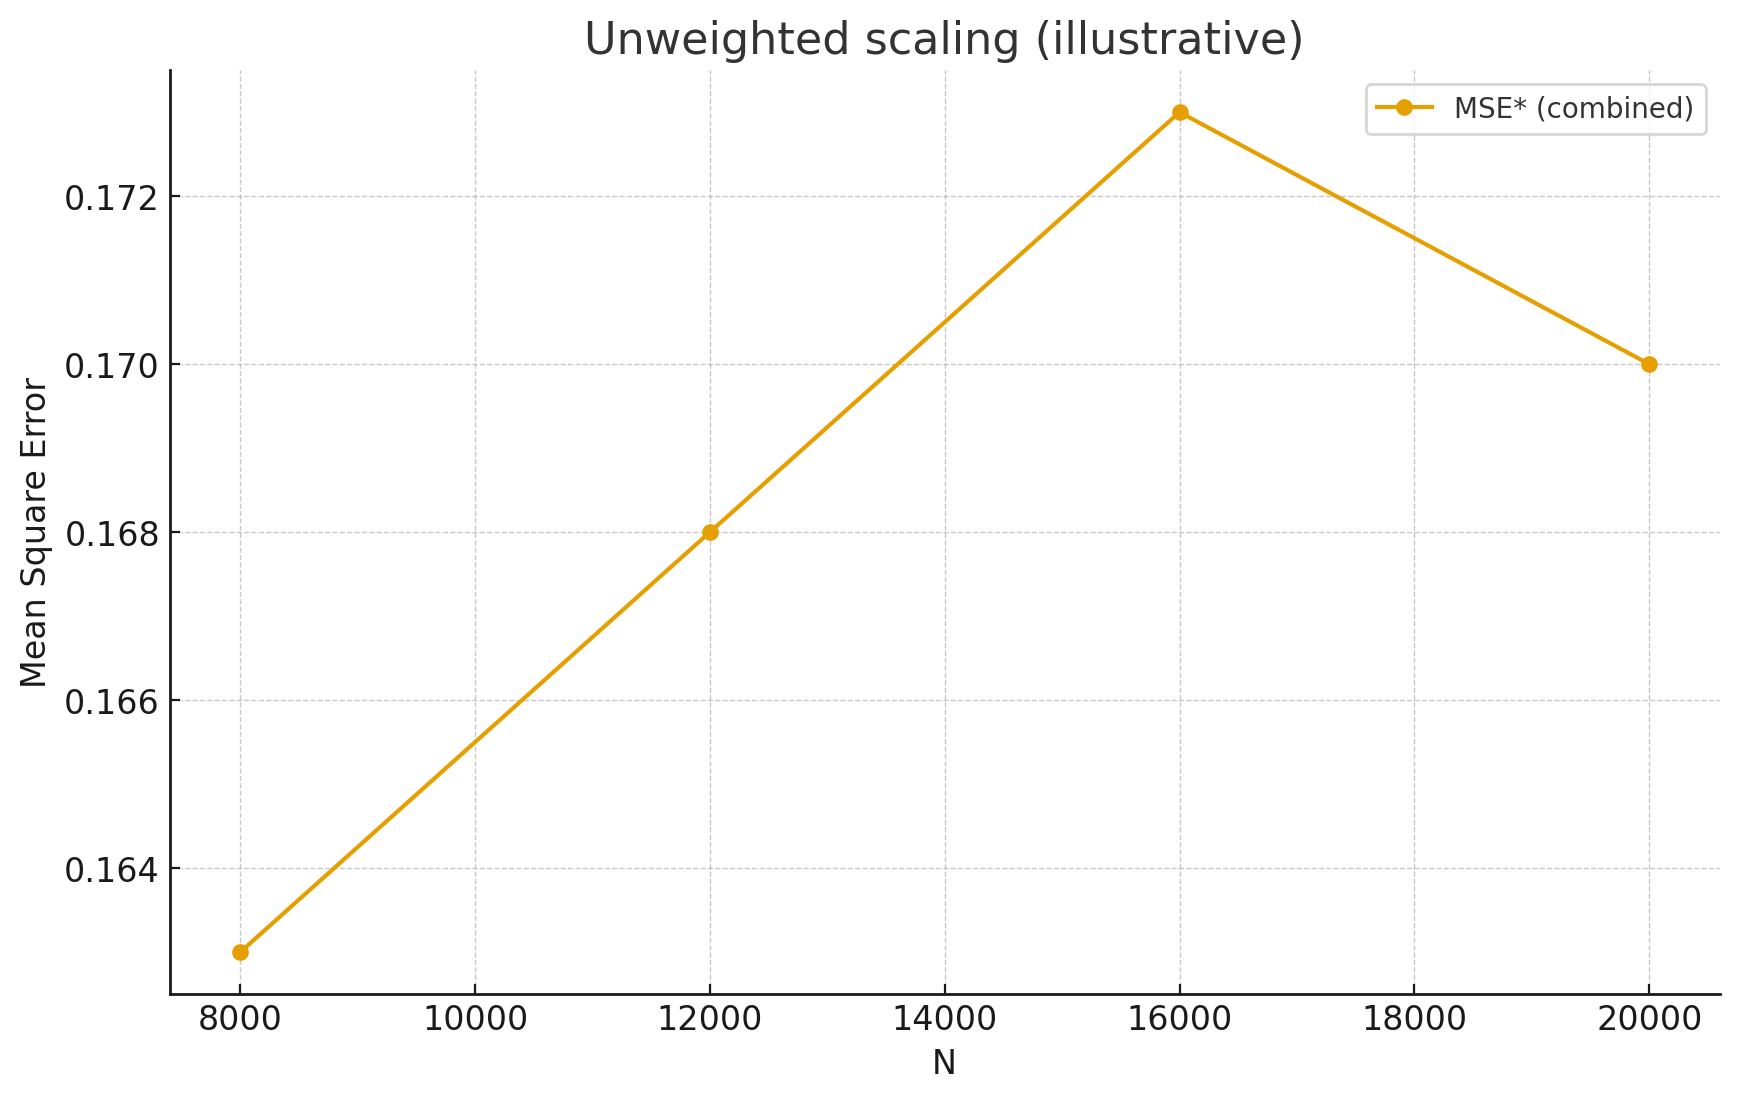
\includegraphics[width=0.8\linewidth]{unweighted_scaling.png}
\caption{Unweighted scaling (reused figure).}
\end{figure}

\begin{figure}[h]
\centering
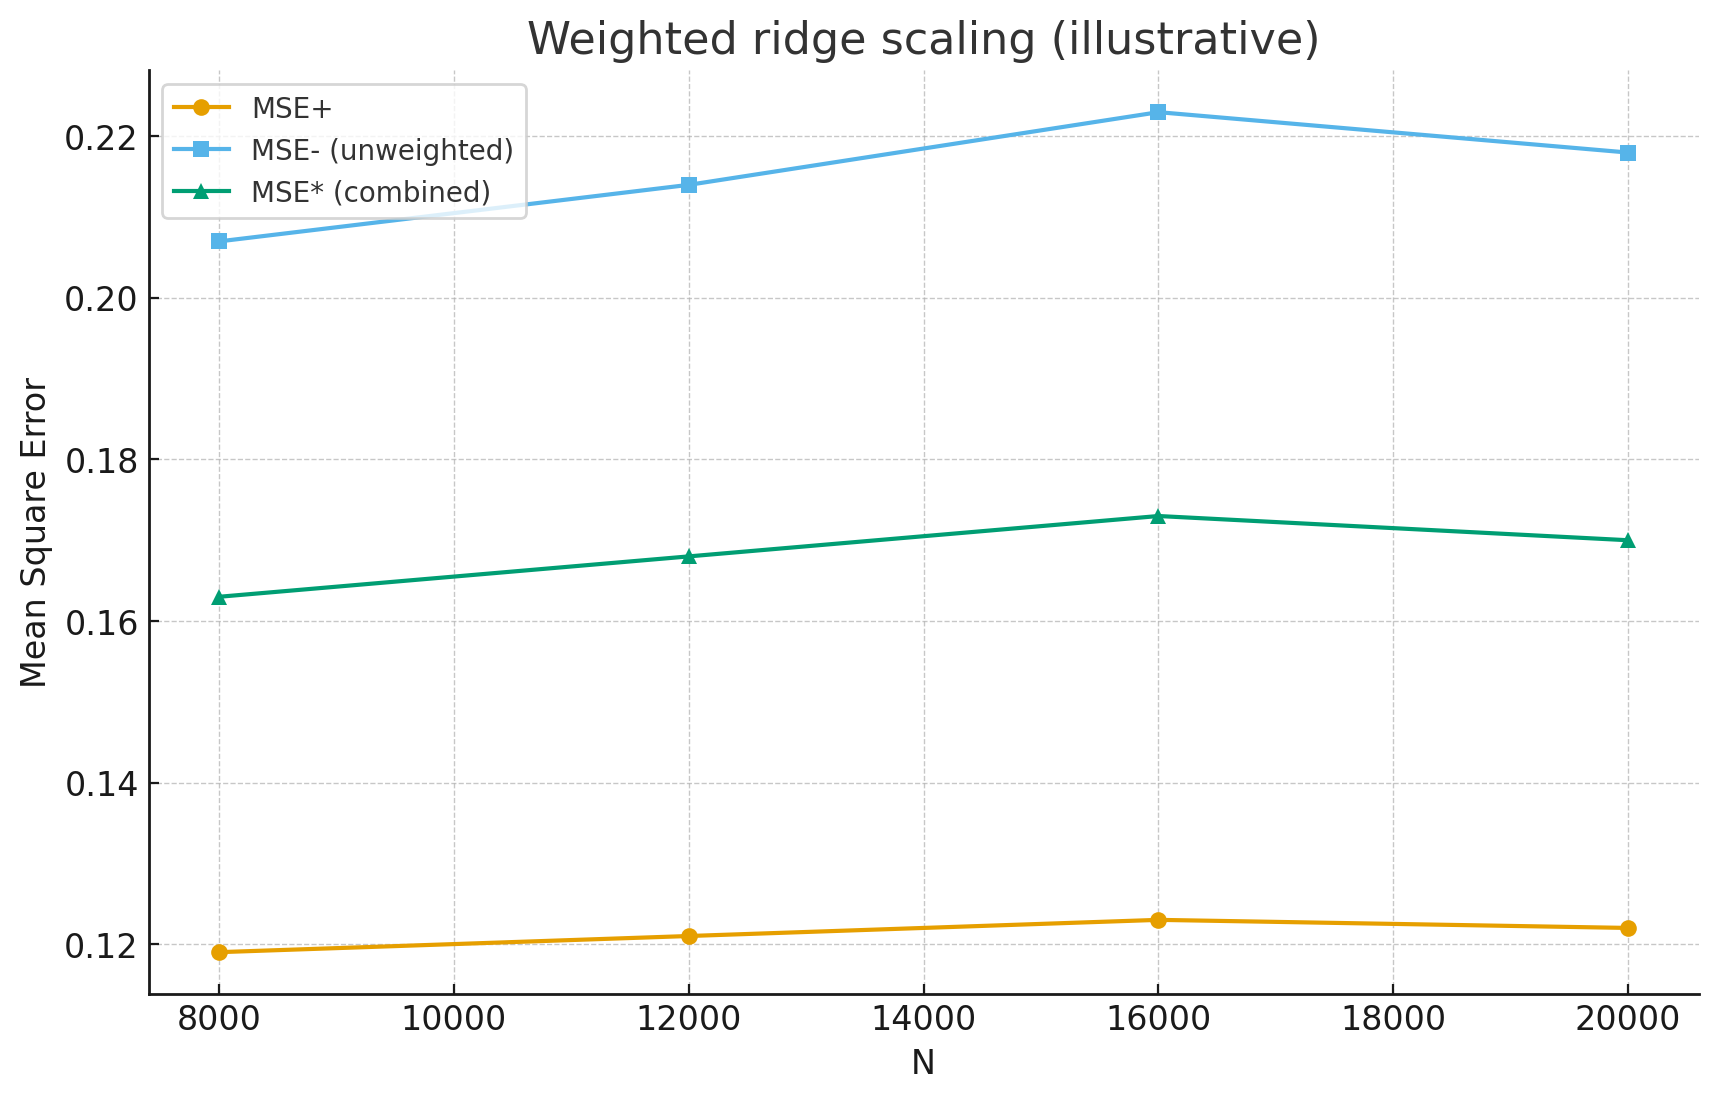
\includegraphics[width=0.8\linewidth]{weighted_scaling.png}
\caption{Weighted ridge scaling (reused figure).}
\end{figure}

\begin{figure}[h]
\centering
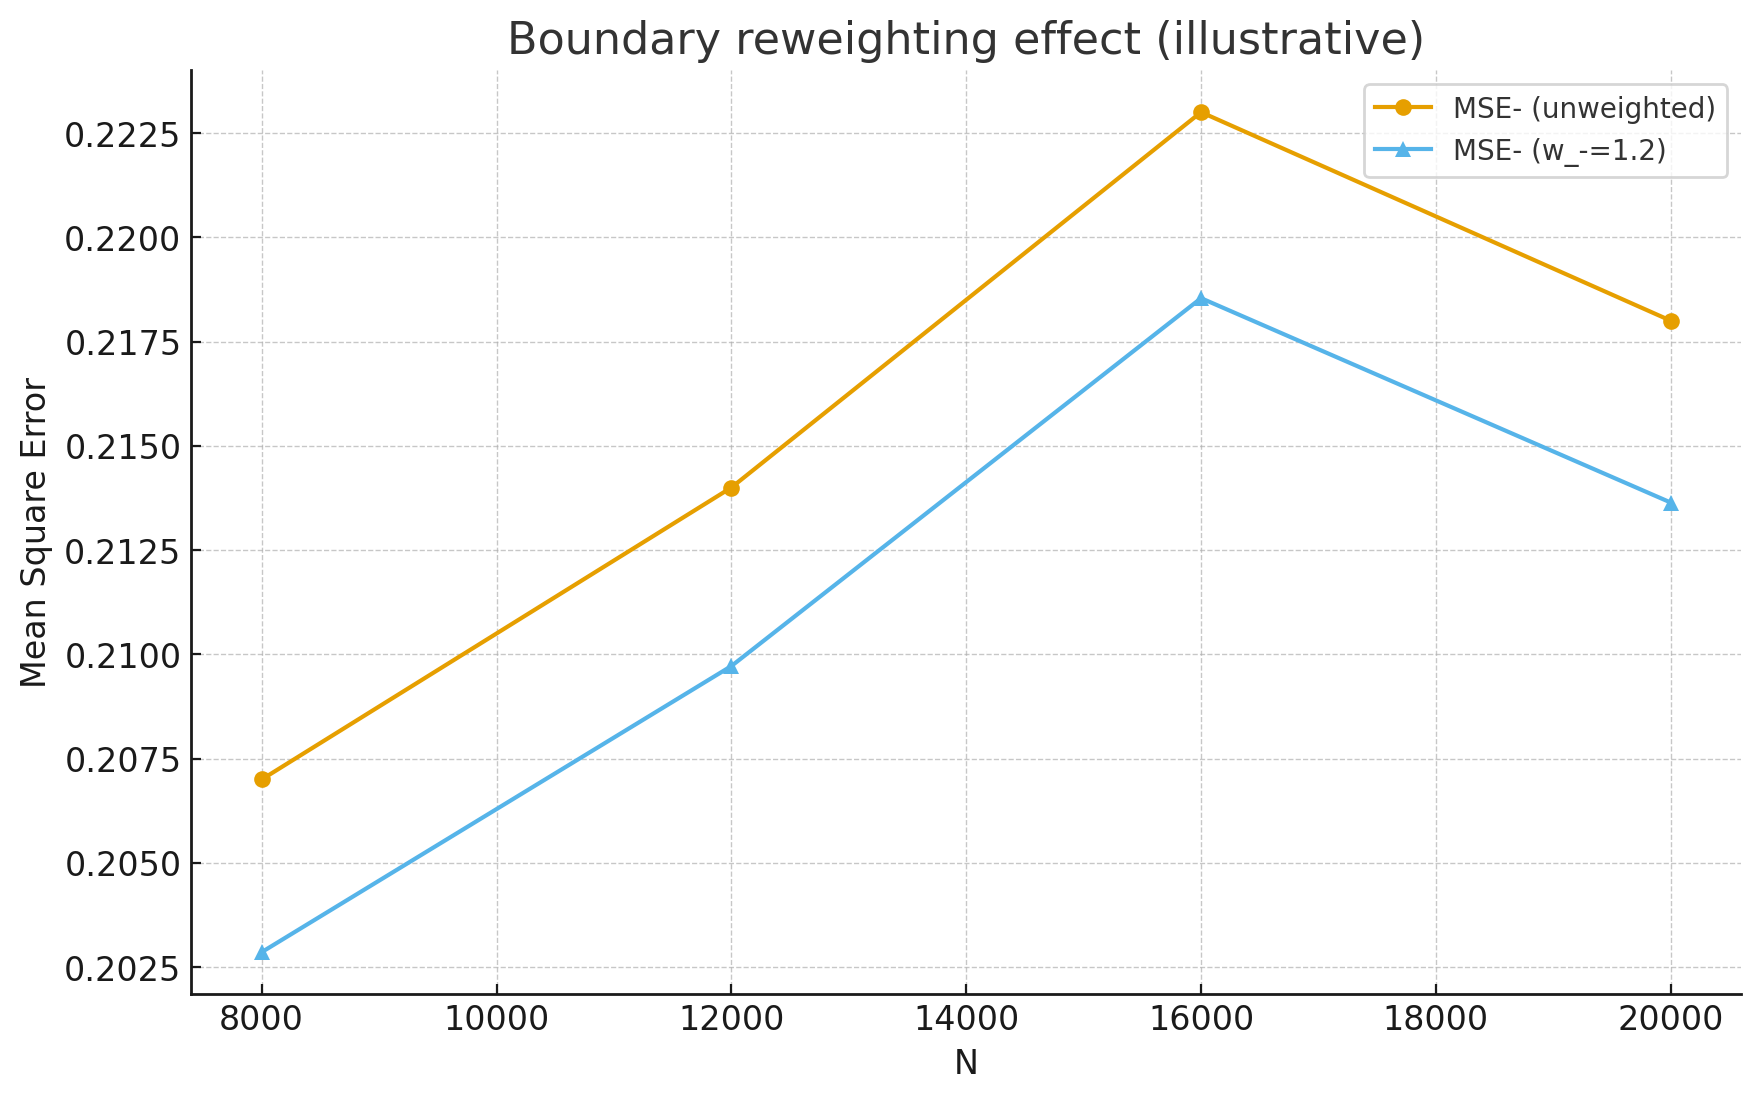
\includegraphics[width=0.8\linewidth]{boundary_reweighting.png}
\caption{Boundary reweighting: $w_- = 1.2$ (reused figure).}
\end{figure}

\section{Scope and Caution}
Inequality~\eqref{eq:hilbert} provides stability control for NB/BD least-squares systems, and the plots
visualize typical behaviour seen in small-scale experiments. This document is not a proof of RH.

\section*{Acknowledgements}
We thank collaborators and correspondents who discussed NB/BD stability and Hilbert-type bounds.

\end{document}